% Point d'avancement tuteur, 14 aout 2026. SEIZE slides.
% Les figures portrait (S19, Z20) ont chacune leur slide, contrainte en HAUTEUR : posees en
% largeur dans le cadre du texte, elles le faisaient deborder de 188 et 200 pt.
% Continuite du 07/08, verifiee point par point :
%   - le call du 07/08 a bute sur une CONFUSION D'ECHELLES (663 M EUR lu comme un SCR) et a
%     demande la CTE en mesure de risque plutot qu'en niveau de couverture -> section A,
%     TROIS slides, placees en tete parce que ce sont les questions du tuteur. La troisieme
%     repond a une demande directe : la slide 6 du 07/08 affichait SIX postures et n'en
%     expliquait aucune, deux d'entre elles (beta = 90 et 99 %) n'etant citees nulle part
%     dans le memoire. La table les definit, et publie le BRUIT DE SIMULATION de chacune ;
%   - le 07/08 laissait implicite le TRAITEMENT des etats de conformite -> section B, deux
%     slides : ce que la conformite deplace, et pourquoi le capital monte plus que la somme ;
%   - le 07/08 annoncait l'allocation Euler/Shapley comme prochain sujet -> section C ;
%   - le 07/08 valorisait deja le capital libere au cout de portage a 6 % -> la slide D
%     l'assume comme une SUITE (et corrige le taux : 4,75 %, directive UE 2025/2), et non
%     comme un axe neuf ;
%   - le 07/08 annoncait la relecture complete -> derniere slide.
% FIL : les questions du dernier call, tranchees ; puis ce qui etait DECLARE devient MESURE.
% Figures : S19, S20, Z20 - aucune n'a servi dans un deck precedent. Les quatre slides des
% sections A et B sont en TABLEAUX et non en figures : U_scr_continu.png aurait convenu au
% fond, mais son ratio de 3,3 pour 1 rend les axes illisibles a la largeur d'une slide 4:3.
% Valeur corrigee au passage (exception au gel d'un deck) : le seuil d'inefficacite passe de
% 76 a 78 %, le script 58 imprimait deux valeurs de la meme grandeur, cf. son commentaire.
\documentclass[11pt]{beamer}
\usetheme{Madrid}
\usecolortheme{seahorse}
\usepackage[utf8]{inputenc}
\usepackage[T1]{fontenc}
\usepackage[french]{babel}
\usepackage{booktabs}
\usepackage{amsmath,amssymb}
\usepackage{eurosym}
\graphicspath{{../vasicek_lab/figures/}{../cascade_qualitative/figures/}{../vasicek_lab/notes/}}
\setbeamertemplate{navigation symbols}{}
\setbeamertemplate{caption}{\raggedright\insertcaption\par}
\setbeamerfont{block title}{size=\small}

\title[Point d'avancement]{Mémoire SCR DORA : point d'avancement}
\subtitle{Trois échelles remises en ordre, et ce qui était déclaré devient mesuré}
\author[K. Kaddouri]{Kélian Kaddouri}
\institute[ENSAE / Nexialog]{ENSAE / Nexialog Consulting}
\date[14/08/2026]{14 août 2026}

\begin{document}

% HARNAIS-HORS-SECTION: page de titre et fil du point. Millesimes, lettres de section et
% renvois internes, aucun resultat de modele.

\begin{frame}
\titlepage
\end{frame}

% =====================================================================
\begin{frame}{Depuis le point du 7 août}
\scriptsize
Le dernier call a buté sur une confusion dont je porte la responsabilité : j'ai présenté un
\textbf{quantile unitaire} là où tu attendais une charge totale. Je commence donc par là, puis
par ta remarque sur la Tail-VaR. Le reste du point est le programme annoncé.
\vspace{1.5mm}
\begin{block}{D'abord tes deux questions, tranchées}
\textbf{(A)} Les \textbf{trois échelles} que nous avions confondues, et le pont entre elles,
désormais calculé et imprimé. Puis la \textbf{mesure de queue}, qui mesure et ne couvre pas.
\end{block}
\vspace{-1mm}
\begin{block}{Ensuite, ce que nous n'avions jamais explicité}
\textbf{(B)} \textbf{Comment les états de conformité sont traités}, et \emph{pourquoi} le
capital monte. Ce n'est pas une pénalité ajoutée au \textsc{scr} : c'est la loi de perte qui
change, sur quatre paramètres, et les quatre ne s'additionnent pas.
\end{block}
\vspace{-1mm}
\begin{block}{Enfin, le fil habituel : ce qui était déclaré devient mesuré}
\textbf{(C)} L'\textbf{allocation aux cinq piliers}, Shapley et Euler.
\textbf{(D)} Le \textbf{coût de portage} poussé jusqu'à sa vraie question, détenir ou
transférer. \textbf{(E)} Les \textbf{deux biais} d'OpRisk, chiffrés. \textbf{(F)} La
\textbf{direction}, corpus élargi et matrice complète. \textbf{(G)} Et une décision à acter :
je propose de \textbf{renoncer à l'élicitation}.
\end{block}
\end{frame}

% =====================================================================
\section*{A. Trois échelles, remises en ordre}

\begin{frame}{Le \texorpdfstring{$663$}{663} M\euro{} n'est pas un SCR, et voici le pont}
\scriptsize
Trois grandeurs ont été comparées comme si elles l'étaient. Elles diffèrent sur \textbf{trois
axes indépendants}, et il ne faut jamais invoquer l'un pour expliquer l'autre.
\vspace{-1mm}
\begin{center}\scriptsize
\begin{tabular}{@{}l l r@{}}
\toprule
\textbf{Objet} & \textbf{Ce que c'est} & \textbf{Valeur} \\
\midrule
$\mathrm{q}_{99{,}5\%}(X)$ & quantile de sévérité, \emph{un} sinistre & $663$ \\
$\mathrm{VaR}_{99{,}5\%}(L)$ & charge \textbf{annuelle agrégée}, secteur & $8\,123$ \\
$\mathrm{VaR}_{99{,}5\%}(L)$ & la même, lue à la taille d'une entité & $169$ \\
\bottomrule
\end{tabular}
\end{center}
\vspace{-1mm}
\begin{block}{Le pont, et il est maintenant imprimé}
À $\lambda=21{,}6$ sinistres par an, atteindre le quantile \emph{annuel} à $99{,}5\,\%$ exige un
quantile \textbf{par sinistre} à $99{,}977\,\%$, soit $4\,530$~M\euro. Le facteur restant,
$\mathbf{1{,}8}$, est l'empreinte de la surdispersion et de la contagion. Aucune non-conformité
là-dedans : c'est de l'\textbf{agrégation}.
\end{block}
\vspace{-1mm}
\begin{block}{Et le sens de l'inégalité s'inverse avec l'échelle}
Au secteur, le capital vaut $\mathbf{12{,}3}$ fois le quantile unitaire. À l'entité,
$\mathbf{0{,}30}$ fois, donc il passe \textbf{en dessous}, la plupart des années n'ayant aucun
sinistre. \textbf{Aucun rapport fixe ne relie les deux objets}, et les comparer ne conclut
jamais. Le mémoire réserve désormais $\mathrm{VaR}$ et $\mathrm{TVaR}$ à l'agrégé, et
$\mathrm{q}$ à la sévérité. Source : script~\texttt{67}, section 1bis.
\end{block}
\end{frame}

% =====================================================================
\begin{frame}{Les six postures, enfin définies, et ce qu'elles supportent}
\scriptsize
La slide de la semaine dernière affichait \textbf{six barres} et n'en expliquait aucune, et deux
d'entre elles n'étaient citées nulle part dans le mémoire. Voici la grille.
\vspace{-1mm}
\begin{center}\scriptsize
\begin{tabular}{@{}l l r r@{}}
\toprule
\textbf{Posture} & \textbf{Ce qu'elle intègre} & \textbf{VaR} & \textbf{bruit} \\
\midrule
Point (\emph{plug-in}) & rien : quantile d'un ajustement ponctuel & $657$ & --- \\
Prédictive & l'incertitude de paramètre, \emph{avant} le quantile & $645$ & $\pm\,7$ \\
Robuste $\beta=90\,\%$ & borne haute de la VaR sur l'ambiguïté de paramètre & $939$ & $\pm\,13$ \\
Robuste $\beta=95\,\%$ & idem, prudence plus élevée & $1\,037$ & $\pm\,9$ \\
Robuste $\beta=99\,\%$ & idem, et la plus bruitée des six & $1\,247$ & $\pm\,24$ \\
Pire-cas de modèle & on ajoute l'ambiguïté de \emph{famille} ($\xi=0{,}90$) & $1\,331$ & --- \\
\bottomrule
\end{tabular}
\end{center}
\vspace{-1mm}
\begin{block}{Deux choses que je n'avais pas vues, et une correction}
\textbf{1.} Les deux \textbf{extrémités} de l'échelle sont \emph{exactes} : le point est le
quantile d'un ajustement unique, le pire-cas celui d'un $\xi$ posé. Tout le bruit est au milieu,
donc dans les postures qui intègrent l'incertitude.\\[2pt]
\textbf{2.} \textbf{La posture la plus prudente est la moins précise} : à $\beta=99\,\%$
l'écart-type de simulation double. Un percentile à $99\,\%$ d'une loi bootstrap de queue lourde
s'estime sur bien moins de tirages utiles. Cela n'invalide pas la posture, cela interdit de la
citer à trois chiffres.\\[2pt]
\textbf{3.} La prédictive était publiée $648$ au chapitre et $645$ sur la figure. Même
estimateur, deux tailles de bootstrap, écart de $3$ pour un bruit de $7$ : \textbf{c'était le
même nombre écrit avec un chiffre de trop}. Toutes les grandeurs simulées de la section sont
désormais publiées avec leur bruit.
\end{block}
\vspace{-1mm}
{\scriptsize Sources : scripts~\texttt{46} et~\texttt{51}.}
\end{frame}

% =====================================================================
\begin{frame}{La mesure de queue sert à mesurer, pas à couvrir}
\scriptsize
Ta remarque était que la Tail-VaR ne doit pas servir de \emph{niveau de couverture}. Le mémoire
y était déjà conforme, mais il ne le disait pas : c'est écrit maintenant.
\vspace{1mm}
\begin{block}{Ce que porte le capital, et ce que porte la CTE}
Le besoin de capital est partout un $\mathrm{VaR}_{99{,}5\%}(L)$ \textbf{centré}, au niveau de
Solvabilité~II. \textbf{Aucune} grandeur de couverture n'est une \textsc{tvar}. La mesure de
queue intervient deux fois, et deux fois comme \emph{diagnostic} : noyau d'allocation d'Euler,
qui répartit un niveau déjà fixé sans le modifier ; et \textbf{indicateur de forme de queue},
par le rapport $\mathrm{TVaR}/\mathrm{VaR}=\mathbf{2{,}1}$ contre l'asymptote
$1/(1-\xi)=2{,}5$. C'est le \emph{rapport} qui informe, pas les deux montants.
\end{block}
\vspace{-1mm}
\begin{block}{Deux raisons de ne pas en faire un niveau, et la seconde tranche}
La proportion d'abord : sur un risque à queues plurielles selon la catégorie d'événement, une
moyenne de queue immobiliserait un capital sans commune mesure avec le niveau réglementaire.
L'\textbf{existence} ensuite : sous la calibration PRC, $\hat\xi=1{,}033>1$, donc l'espérance
est infinie et \textbf{la mesure n'existe pas}. Une couverture qui cesse d'être définie selon la
source de sévérité ne peut pas porter un capital ; le même objet lu comme diagnostic reste
informatif, puisque sa divergence \emph{est} l'information.
\end{block}
\vspace{-1mm}
{\scriptsize Deux limites déclarées au passage, de sens opposés : l'\textbf{attritionnel} est
absent de la base, tronquée à son seuil de collecte, ce qui \emph{sous-estime} ; et la sévérité
n'est \textbf{pas plafonnée} à l'échelle d'entité, élasticité à la taille $0{,}087$, ce qui
\emph{majore} le niveau d'entité. Elles ne se compensent pas.
Sources : scripts~\texttt{51}, \texttt{60} et~\texttt{67}.}
\end{frame}

% =====================================================================
\section*{B. Les états de conformité, et pourquoi le capital monte}

\begin{frame}{Ce que la conformité déplace, exactement}
\scriptsize
La question mérite d'être posée à l'envers de l'intuition courante. La non-conformité
\textbf{n'ajoute aucune pénalité} au \textsc{scr} : elle déplace quatre paramètres de la loi de
perte, et le capital monte parce que \emph{la loi a changé}, pas parce qu'un coefficient s'y
applique.
\vspace{-1mm}
\begin{center}\scriptsize
\begin{tabular}{@{}l l l r@{}}
\toprule
\textbf{Canal} & \textbf{Ce que DORA y observe} & \textbf{Paramètre} & \textbf{C $\to$ NC} \\
\midrule
Fréquence & \textsc{kpi} d'entrée d'incidents & $\lambda$ & $21{,}6 \to 53{,}6$ \\
Détection & délai P2, confinement P3 & $p_u$ & $0{,}128 \to 0{,}181$ \\
Propagation & canal $W$, non identifié & $g$ & $0{,}45 \to 0{,}90$ \\
Accumulation & concentration des tiers P4 & $\varphi_{cs}$ & $0 \to 0{,}68$ \\
\bottomrule
\end{tabular}
\end{center}
\vspace{-1mm}
\begin{block}{Deux canaux se calibrent, deux se bornent, et la distinction est le point}
Fréquence et détection s'adossent à des \textsc{kpi} \textbf{mesurables} : ce sont les leviers
de remédiation actionnables. Propagation et accumulation ne sont pas identifiées : elles disent
l'\textbf{incertitude}, et se résorbent par la donnée du registre DORA, pas par une action.
Confondre les deux, c'est promettre une remédiation là où l'on n'a qu'une borne.
\end{block}
\vspace{-1mm}
\begin{block}{Et les trois états ne sont qu'une grille de lecture}
Le \textsc{scr} est une fonction \emph{continue} du score de conformité $q$ : à $g$ maintenu au
niveau non conforme, il décroît régulièrement de $16\,847$ à $7\,987$~M\euro, soit
$\mathbf{-53\,\%}$. Découper en trois, ou en cinq, est une commodité de lecture et non un choix
de modèle. Sources : scripts~\texttt{25} et~\texttt{43}.
\end{block}
\end{frame}

% =====================================================================
\begin{frame}{Pourquoi le capital monte, et plus que la somme des canaux}
\scriptsize
\begin{columns}[t]
\begin{column}{0.45\linewidth}
\centering
\textbf{Les deux repères}\\[3pt]
\begin{tabular}{@{}l r@{}}
\toprule
\textbf{État} & \textbf{SCR} \\
\midrule
Conforme (cible DORA) & $6\,049$ \\
Non conforme & $\mathbf{20\,188}$ \\
\midrule
$\Delta_{\text{DORA}}$ & $\mathbf{14\,139}$ \\
\bottomrule
\end{tabular}\\[4pt]
{\scriptsize Soit un facteur $\mathbf{3{,}3}$, à sévérité de base et à échelle inchangées.}
\end{column}
\begin{column}{0.52\linewidth}
\centering
\textbf{Un canal à la fois}\\[3pt]
\begin{tabular}{@{}l r r@{}}
\toprule
\textbf{Canal} & \textbf{$\Delta$SCR} & \textbf{statut} \\
\midrule
Fréquence & $\mathbf{4\,328}$ & calibrable \\
Accumulation P4 & $1\,728$ & borne \\
Propagation $W$ & $1\,633$ & borne \\
Détection P2/P3 & $1\,448$ & calibrable \\
\midrule
\textbf{somme} & $9\,138$ & \\
\bottomrule
\end{tabular}
\end{column}
\end{columns}
\vspace{1mm}
\begin{block}{L'écart entre $9\,138$ et $14\,139$ est le résultat, pas un résidu}
\textbf{$+5\,001$~M\euro{} d'interaction, soit $+35\,\%$} : la cascade est
\textbf{super-additive}, et c'est mécanique. À queue lourde le quantile est porté par un
sinistre unique, si bien que relever à la fois la fréquence, la probabilité de franchir le seuil
et la force de propagation ne produit pas quatre effets qui s'ajoutent mais un effet
\emph{composé} ; et la contagion transforme des défaillances isolées en choc commun.\\[3pt]
D'où ce qu'on peut dire et ce qu'on ne peut pas. \textbf{Un forfait plat ne peut pas
représenter ce mécanisme}, faute d'un canal où l'inscrire. Et \textbf{on n'additionne pas les
quatre leviers} pour chiffrer une remédiation partielle : c'est justement le résultat.
\end{block}
\end{frame}

% =====================================================================
\section*{C. L'allocation aux cinq piliers}

\begin{frame}{Shapley et Euler : la suite des \texorpdfstring{$5\,001$}{5001} M\euro{} d'interaction}
\scriptsize
Deux questions, deux règles. \emph{Qui porte le surcoût ?} appelle une attribution par pilier
\textbf{source}, composant avec l'interaction puisque les marginaux ne somment pas au total :
c'est Shapley. \emph{Où loge le capital ?} appelle une allocation par pilier \textbf{touché},
dont les parts somment au total : c'est Euler.
\vspace{-2mm}
\begin{center}\scriptsize
\begin{tabular}{@{}l rrr@{}}
\toprule
\textbf{Pilier} & \textbf{marginal} & $\boldsymbol{\varphi_j}$ \textbf{(Shapley)} & \textbf{part} \\
\midrule
P1 gouvernance & $3\,481$ & $\mathbf{3\,717}$ & $34\,\%$ \\
P4 tiers & $2\,658$ & $2\,810$ & $26\,\%$ \\
P2 incidents & $1\,634$ & $1\,867$ & $17\,\%$ \\
P3 tests & $1\,094$ & $1\,484$ & $14\,\%$ \\
P5 partage & $665$ & $1\,048$ & $10\,\%$ \\
\midrule
\textbf{somme} & $9\,531$ & $\mathbf{10\,927}$ & $100\,\%$ \\
\bottomrule
\end{tabular}
\end{center}
\vspace{-1mm}
\begin{block}{Ce qu'il faut regarder, et la limite que j'assume}
\textbf{Le test non trivial n'est pas le classement mais la déformation.} Le classement
reproduit ROOT, ce qui est en partie \emph{mécanique} (les amorces sont semées
proportionnellement à ROOT). Ce qui ne l'est pas : la part de P1 ($34\,\%$) \textbf{excède} sa
part d'amorce ($30\,\%$), effet propre de la propagation, et les $\mathbf{+1\,395}$~M\euro{}
redistribués sont \textbf{intégralement} un produit de la cascade.\\[3pt]
\textbf{Côté Euler}, les parts \emph{moyennes} sont stables (P2 $23\,\%$, P4 $22\,\%$, P1
$20\,\%$), mais à $\xi\approx0{,}6>0{,}5$ la sévérité est de \textbf{variance infinie} : le
classement de queue bascule d'une résolution à l'autre. Je rapporte donc la queue du périmètre
PRC et tiens celle d'OpRisk pour indicative.
\end{block}
\vspace{-1mm}
{\scriptsize Sources : scripts~\texttt{16b}, \texttt{20}, \texttt{20b}, \texttt{43}
et~\texttt{67}.}
\end{frame}

% =====================================================================
\section*{D. Ce que le capital coûte}

\begin{frame}{Détenir ou transférer}
\scriptsize
La dernière fois, nous valorisions le capital libéré \emph{au seul coût de portage}
($848$~M\euro/an) au taux de $6\,\%$. Le taux est désormais $\mathbf{4{,}75\,\%}$ (directive
(UE)~2025/2), et le portage se retourne en une \emph{question} : si détenir coûte, vaut-il
mieux \textbf{transférer} ?

\alert{\textbf{Le SCR d'entité a changé : $488 \to 169$~M\euro.}} Nous lisions la fréquence
sur les firmes OpRisk à au moins dix événements, dont les actifs médians valent \textbf{dix-neuf
fois} notre entité, et ce seau est en plus défini par un filtre sur la grandeur qu'on estime.
$\lambda$ est maintenant estimé comme une \emph{fonction} de la taille et lu à la bonne taille
($0{,}092$), et la correction de sévérité déjà mesurée est enfin composée. À assumer : la
coïncidence avec la Formule Standard ($450$) \textbf{ne survit pas}, elle venait du seuil.
\vspace{2mm}
\begin{block}{Trois chiffres, et une borne}
À l'échelle d'entité, détenir coûte $\mathbf{8{,}0}$~M\euro/an contre $3{,}6$ de sinistralité
attendue, soit $\mathbf{2{,}2}$ fois. Multiple de capital $\mathbf{47}$ à l'entité contre
$8{,}3$ au secteur. Le traité optimal ($L^\star=\mathrm{SCR}=169$) ramène le coût à $2{,}9$,
soit $\mathbf{-64\,\%}$. \textbf{Borne supérieure} : il faudrait $\mathbf{78\,\%}$
d'inefficacité, capacité et contrepartie comprises, pour renverser la conclusion.
\end{block}
\vspace{-1mm}
{\scriptsize Sources : scripts~\texttt{50}, \texttt{58} et~\texttt{60}.}
\end{frame}

% =====================================================================
% LA FIGURE A SA PROPRE SLIDE, ET ELLE EST CONTRAINTE PAR LA HAUTEUR. S19 est un portrait
% de ratio 1,29 : posee a 0,60 de la LARGEUR elle mesurait 85 mm de haut pour 74 mm utiles,
% et le cadre debordait de 188 pt, soit 6,6 cm hors de la slide. Sur un format 4:3 une
% figure portrait ne peut se dimensionner qu'en hauteur.
\begin{frame}{Détenir ou transférer, en image}
\begin{center}
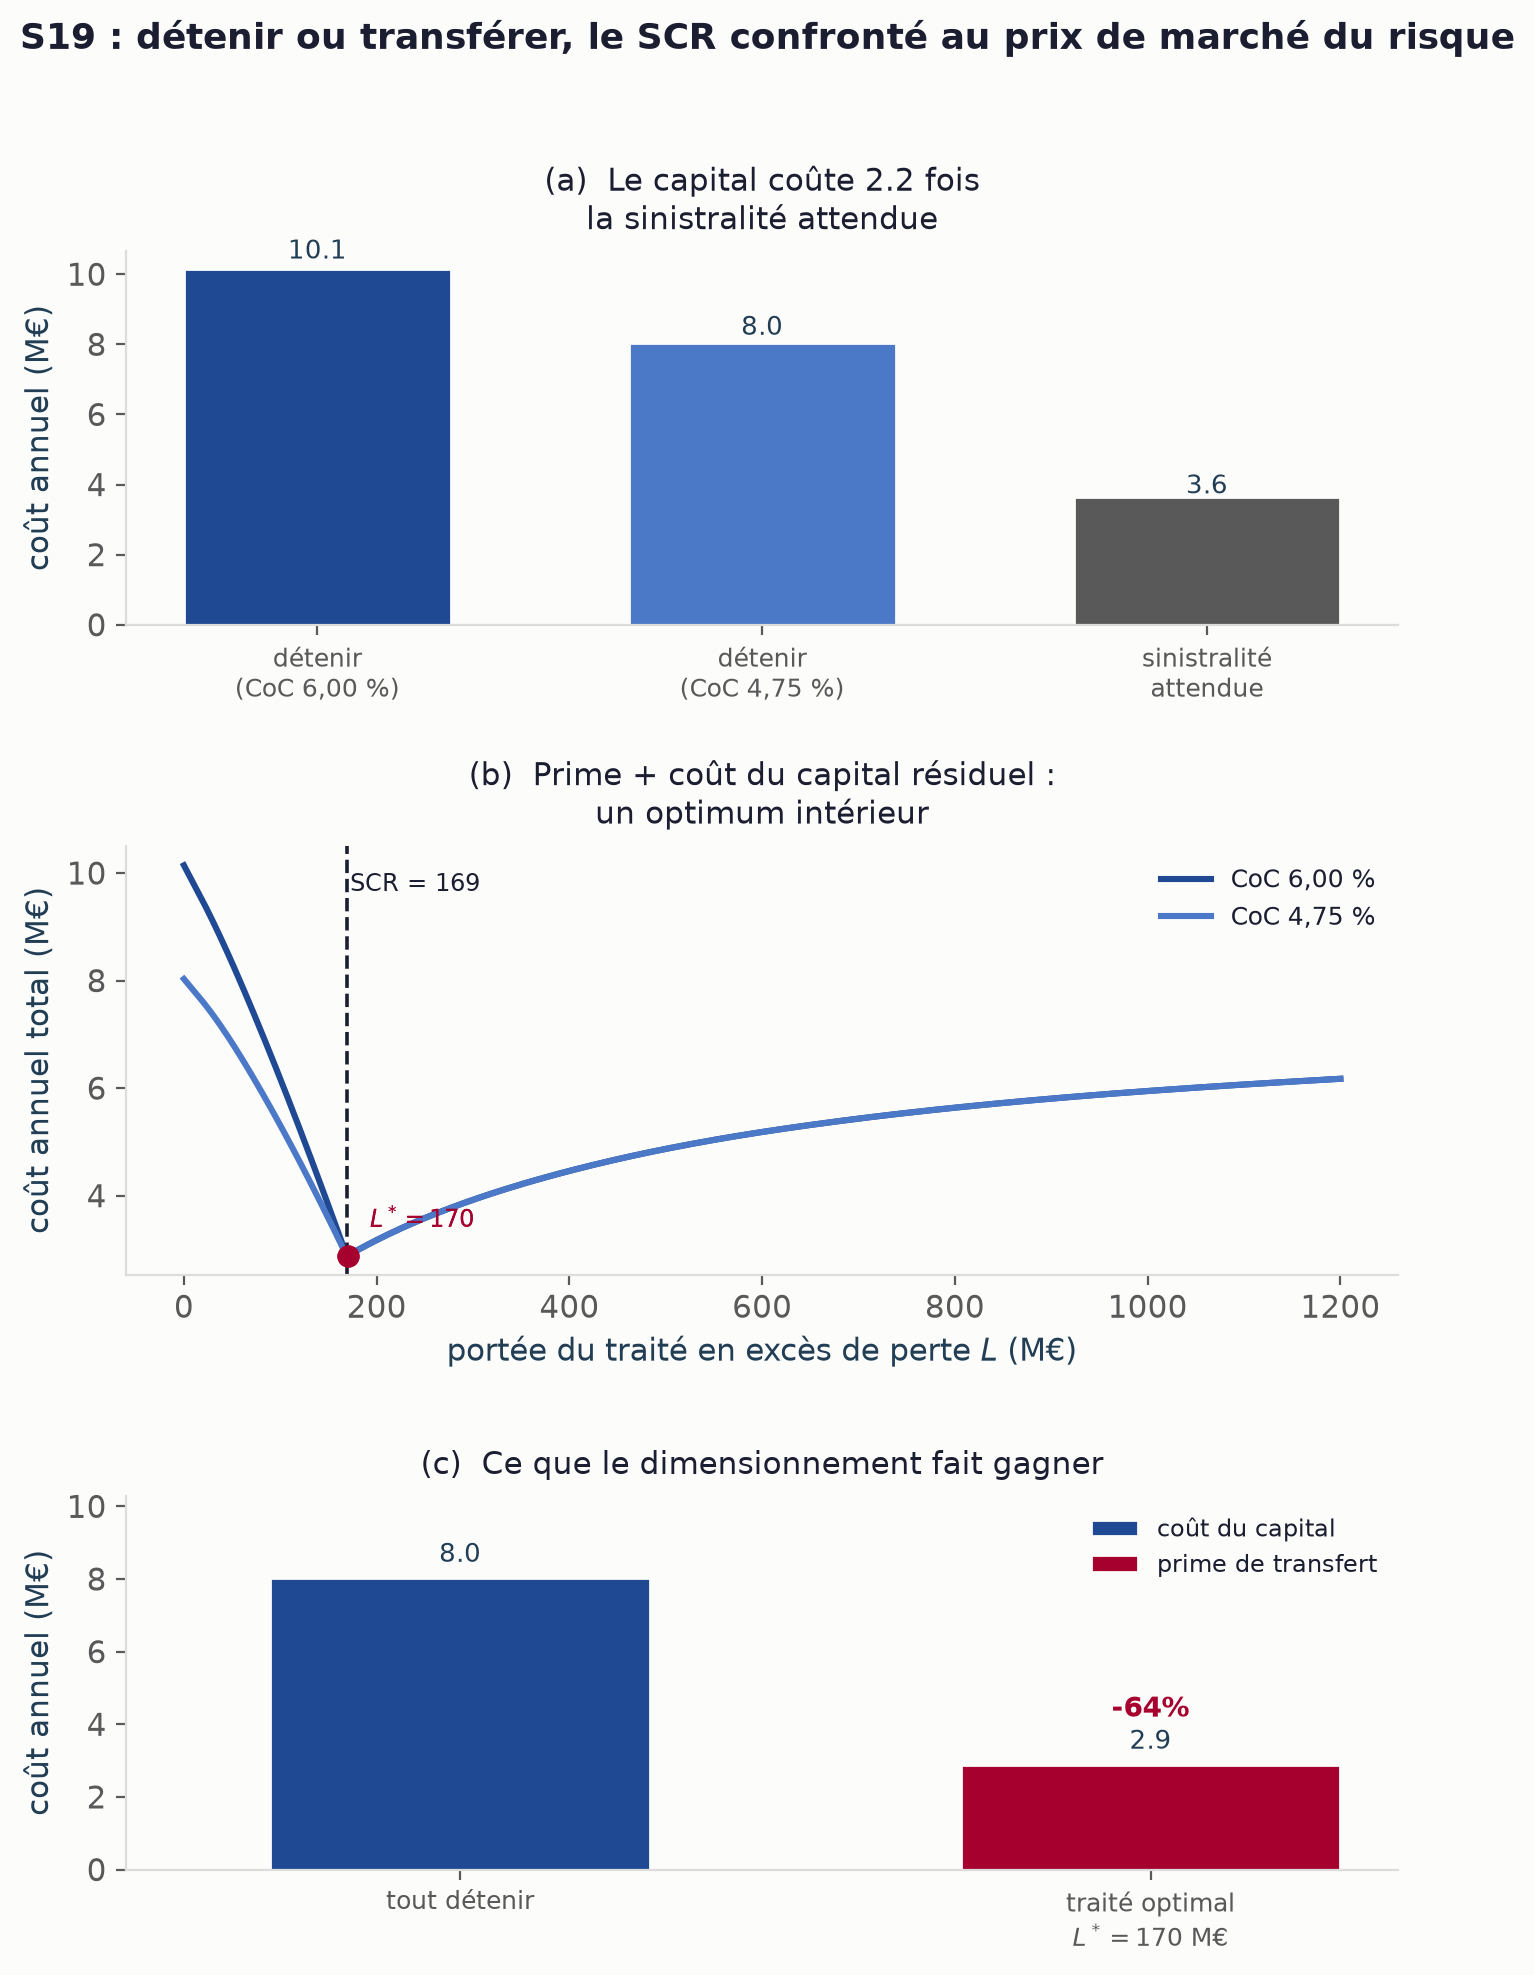
\includegraphics[height=0.80\textheight]{S19_detenir_ou_transferer.png}
\end{center}
\end{frame}

% =====================================================================
\section*{E. Deux biais enfin chiffrés}

\begin{frame}{Les deux biais que nous déclarions}
\scriptsize
Déclarer un biais ne coûte rien, le mesurer engage. Les deux qu'on nous oppose le plus se
mesurent \textbf{avec la base elle-même} : elle porte les actifs de la firme sinistrée, et la
date de saisie en plus de l'année de survenance.
\begin{center}
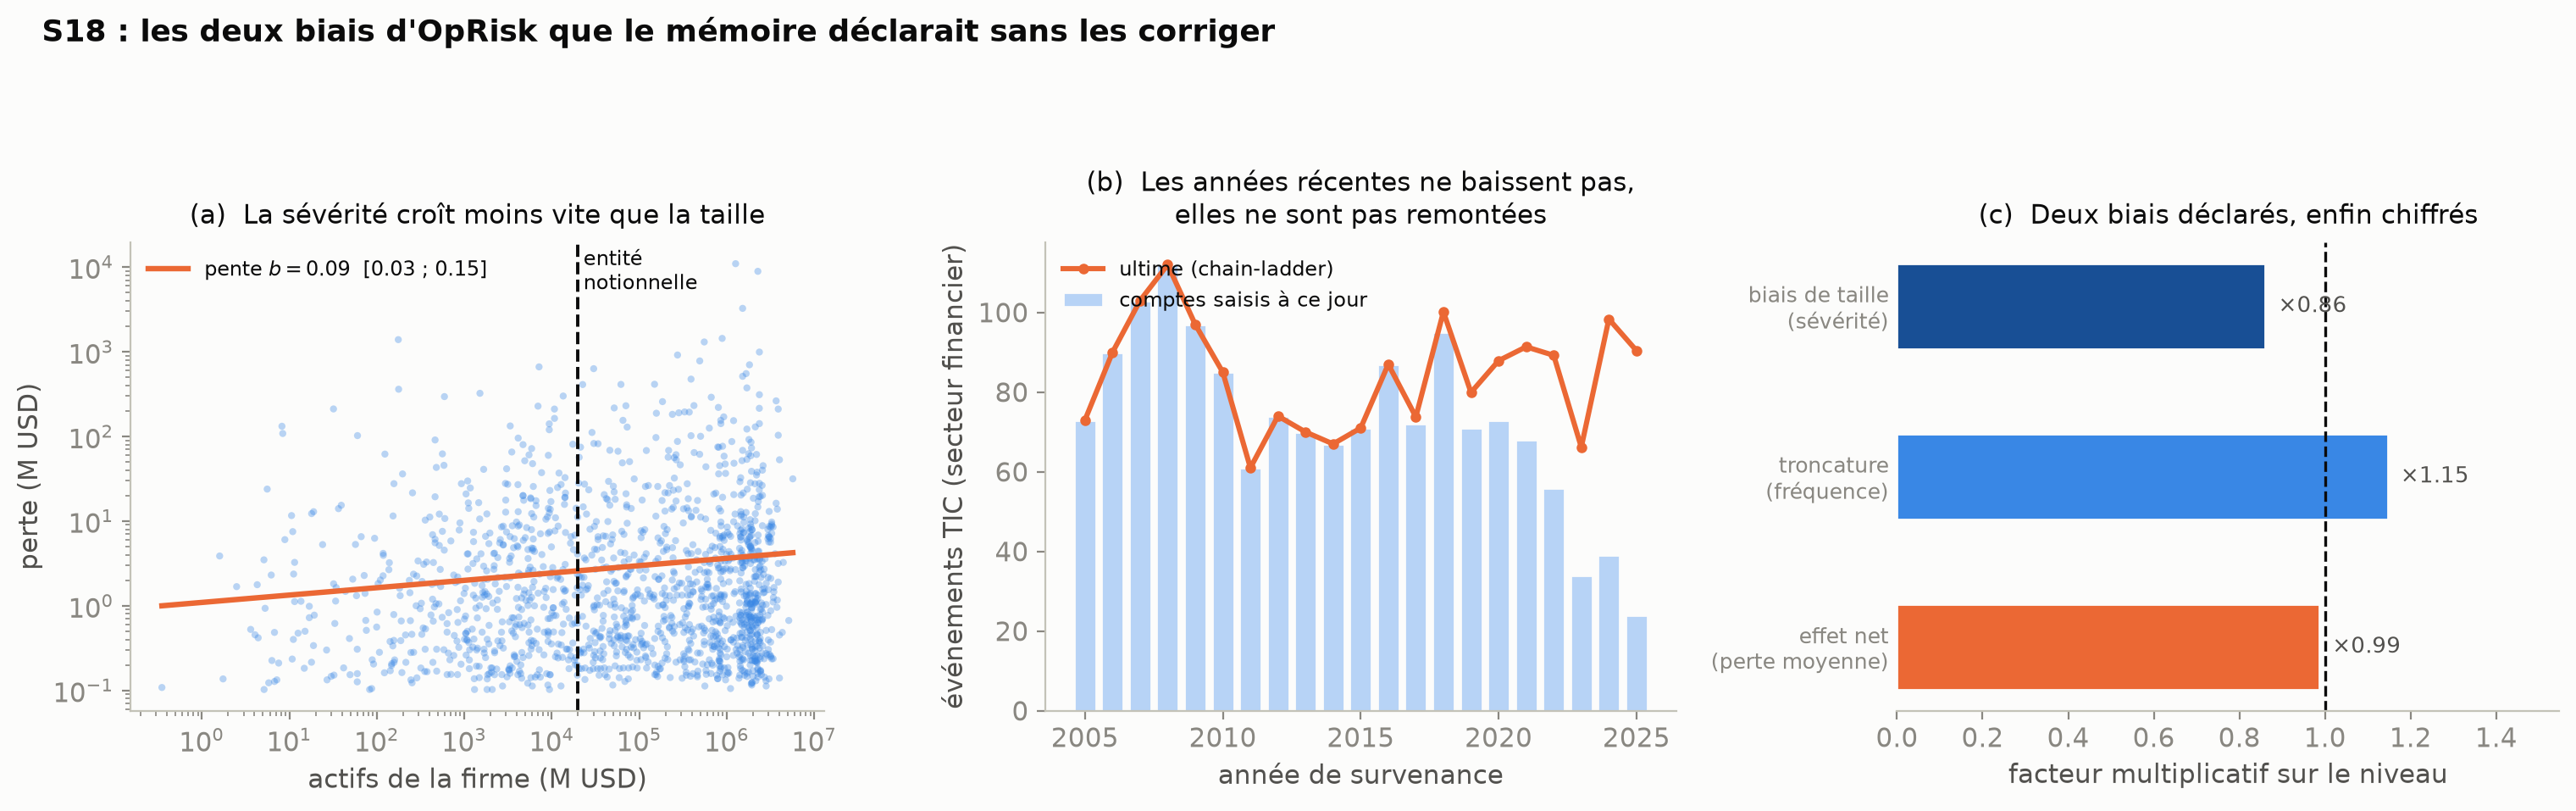
\includegraphics[width=0.83\linewidth]{S20_biais_taille_troncature.png}
\end{center}
\vspace{-2mm}
\begin{block}{Taille : un septième, pas un facteur dix}
Élasticité brute $0{,}042$ ($R^2=0{,}005$), \emph{aplatie} par le seuil de collecte, une petite
firme n'entrant qu'avec une perte anormale. Corrigée par maximum de vraisemblance tronqué :
$\mathbf{0{,}087}$ $[0{,}026;0{,}148]$, soit une sévérité transposée $\times 0{,}86$.
\end{block}
\vspace{-1mm}
\begin{block}{Troncature : la baisse après 2022 n'existe pas}
Délai médian de remontée \textbf{trois ans}. Au chain-ladder, les $97$ événements de
2023--2025 deviennent $\mathbf{255}$, soit $\mathbf{+163\,\%}$, \emph{au-dessus} de la moyenne
historique. \emph{Sources : scripts~\texttt{08} et~\texttt{57}.}
\end{block}
\end{frame}

% =====================================================================
\begin{frame}{Le résultat que je n'attendais pas}
\small
Les deux corrections vont en sens opposés. Sur la \textbf{perte moyenne}, elles se
\textbf{compensent presque exactement} :
\[
  0{,}861 \times 1{,}147 \;=\; 0{,}987 ,
\]
soit un effet net de $1{,}3\,\%$, inférieur à l'incertitude d'estimation de chacune prise
isolément.
\vspace{2mm}
\begin{block}{Sur le capital, elles ne se compensent pas}
À queue lourde, la VaR $99{,}5\,\%$ obéit au \textbf{principe du grand saut unique} : elle
répond à la \emph{sévérité} bien plus qu'à la \emph{fréquence}. La correction de taille agit
sur la sévérité et se transmet donc au quantile ; celle de troncature agit sur la fréquence et
s'y transmet mal.
\end{block}
\vspace{1mm}
\begin{block}{Ce qu'il faut en retenir}
\textbf{Deux biais qui s'annulent sur l'espérance peuvent ne pas s'annuler sur le quantile, et
c'est le quantile qui fait le SCR.} Une compensation constatée en moyenne n'autorise donc pas
à ignorer les deux biais. \emph{Sources : scripts~\texttt{57} et~\texttt{60}.}
\end{block}
\end{frame}

% =====================================================================
\section*{F. La direction, sur la matrice complète}

\begin{frame}{Corpus élargi, et matrice ordonnée}
\scriptsize
Deux objections restaient. Le signal tenait-il au \emph{choix} des sept incidents ? Et le
codage ne comparait que le \emph{sens} dans une paire, sans rien dire de l'\textbf{amplitude}.
En déclarant aussi les piliers défaillants \emph{sans} propagation, on obtient le dénominateur
qui manquait : $p_{jk}\sim\mathrm{Beta}(1+m_{jk},\,1+N_j-m_{jk})$.
\vspace{-1mm}
\begin{center}
\begin{tabular}{@{}l r@{\hskip 1.4em}l r@{}}
\toprule
Corpus initial ($7$) & $z=+3{,}93$ & Sources \emph{primaires} seules & $z=+4{,}08$ \\
\textbf{Étendu} ($10$, $22$ trans.) & $\mathbf{z=+5{,}12}$ & Perspective \emph{entité} seule & $z=+3{,}62$ \\
\bottomrule
\end{tabular}
\end{center}
\vspace{1mm}
\begin{block}{Le résultat est asymétrique, et je le présente comme tel}
$\mathbf{12}$ liens sur $20$ ont un crédible entièrement \emph{sous} $0{,}5$, \textbf{aucun}
au-dessus. J'établis très bien \emph{où la contagion ne va pas}, pas où elle va fort. La
corrélation avec le classeur n'est pas significative ($\rho=+0{,}31$, $p=0{,}19$).
\textbf{Le corpus établit un ordre, pas une magnitude.}
\end{block}
\vspace{-1mm}
{\scriptsize Sources : scripts~\texttt{53}, \texttt{59} et~\texttt{64}.}
\end{frame}

% =====================================================================
% MEME CAUSE, MEME REMEDE QUE POUR S19. Z20 est un portrait de ratio 1,03 : a 0,85 de la
% largeur elle mesurait 94 mm de haut, et le cadre debordait de 200 pt.
\begin{frame}{La matrice ordonnée, en image}
\begin{center}
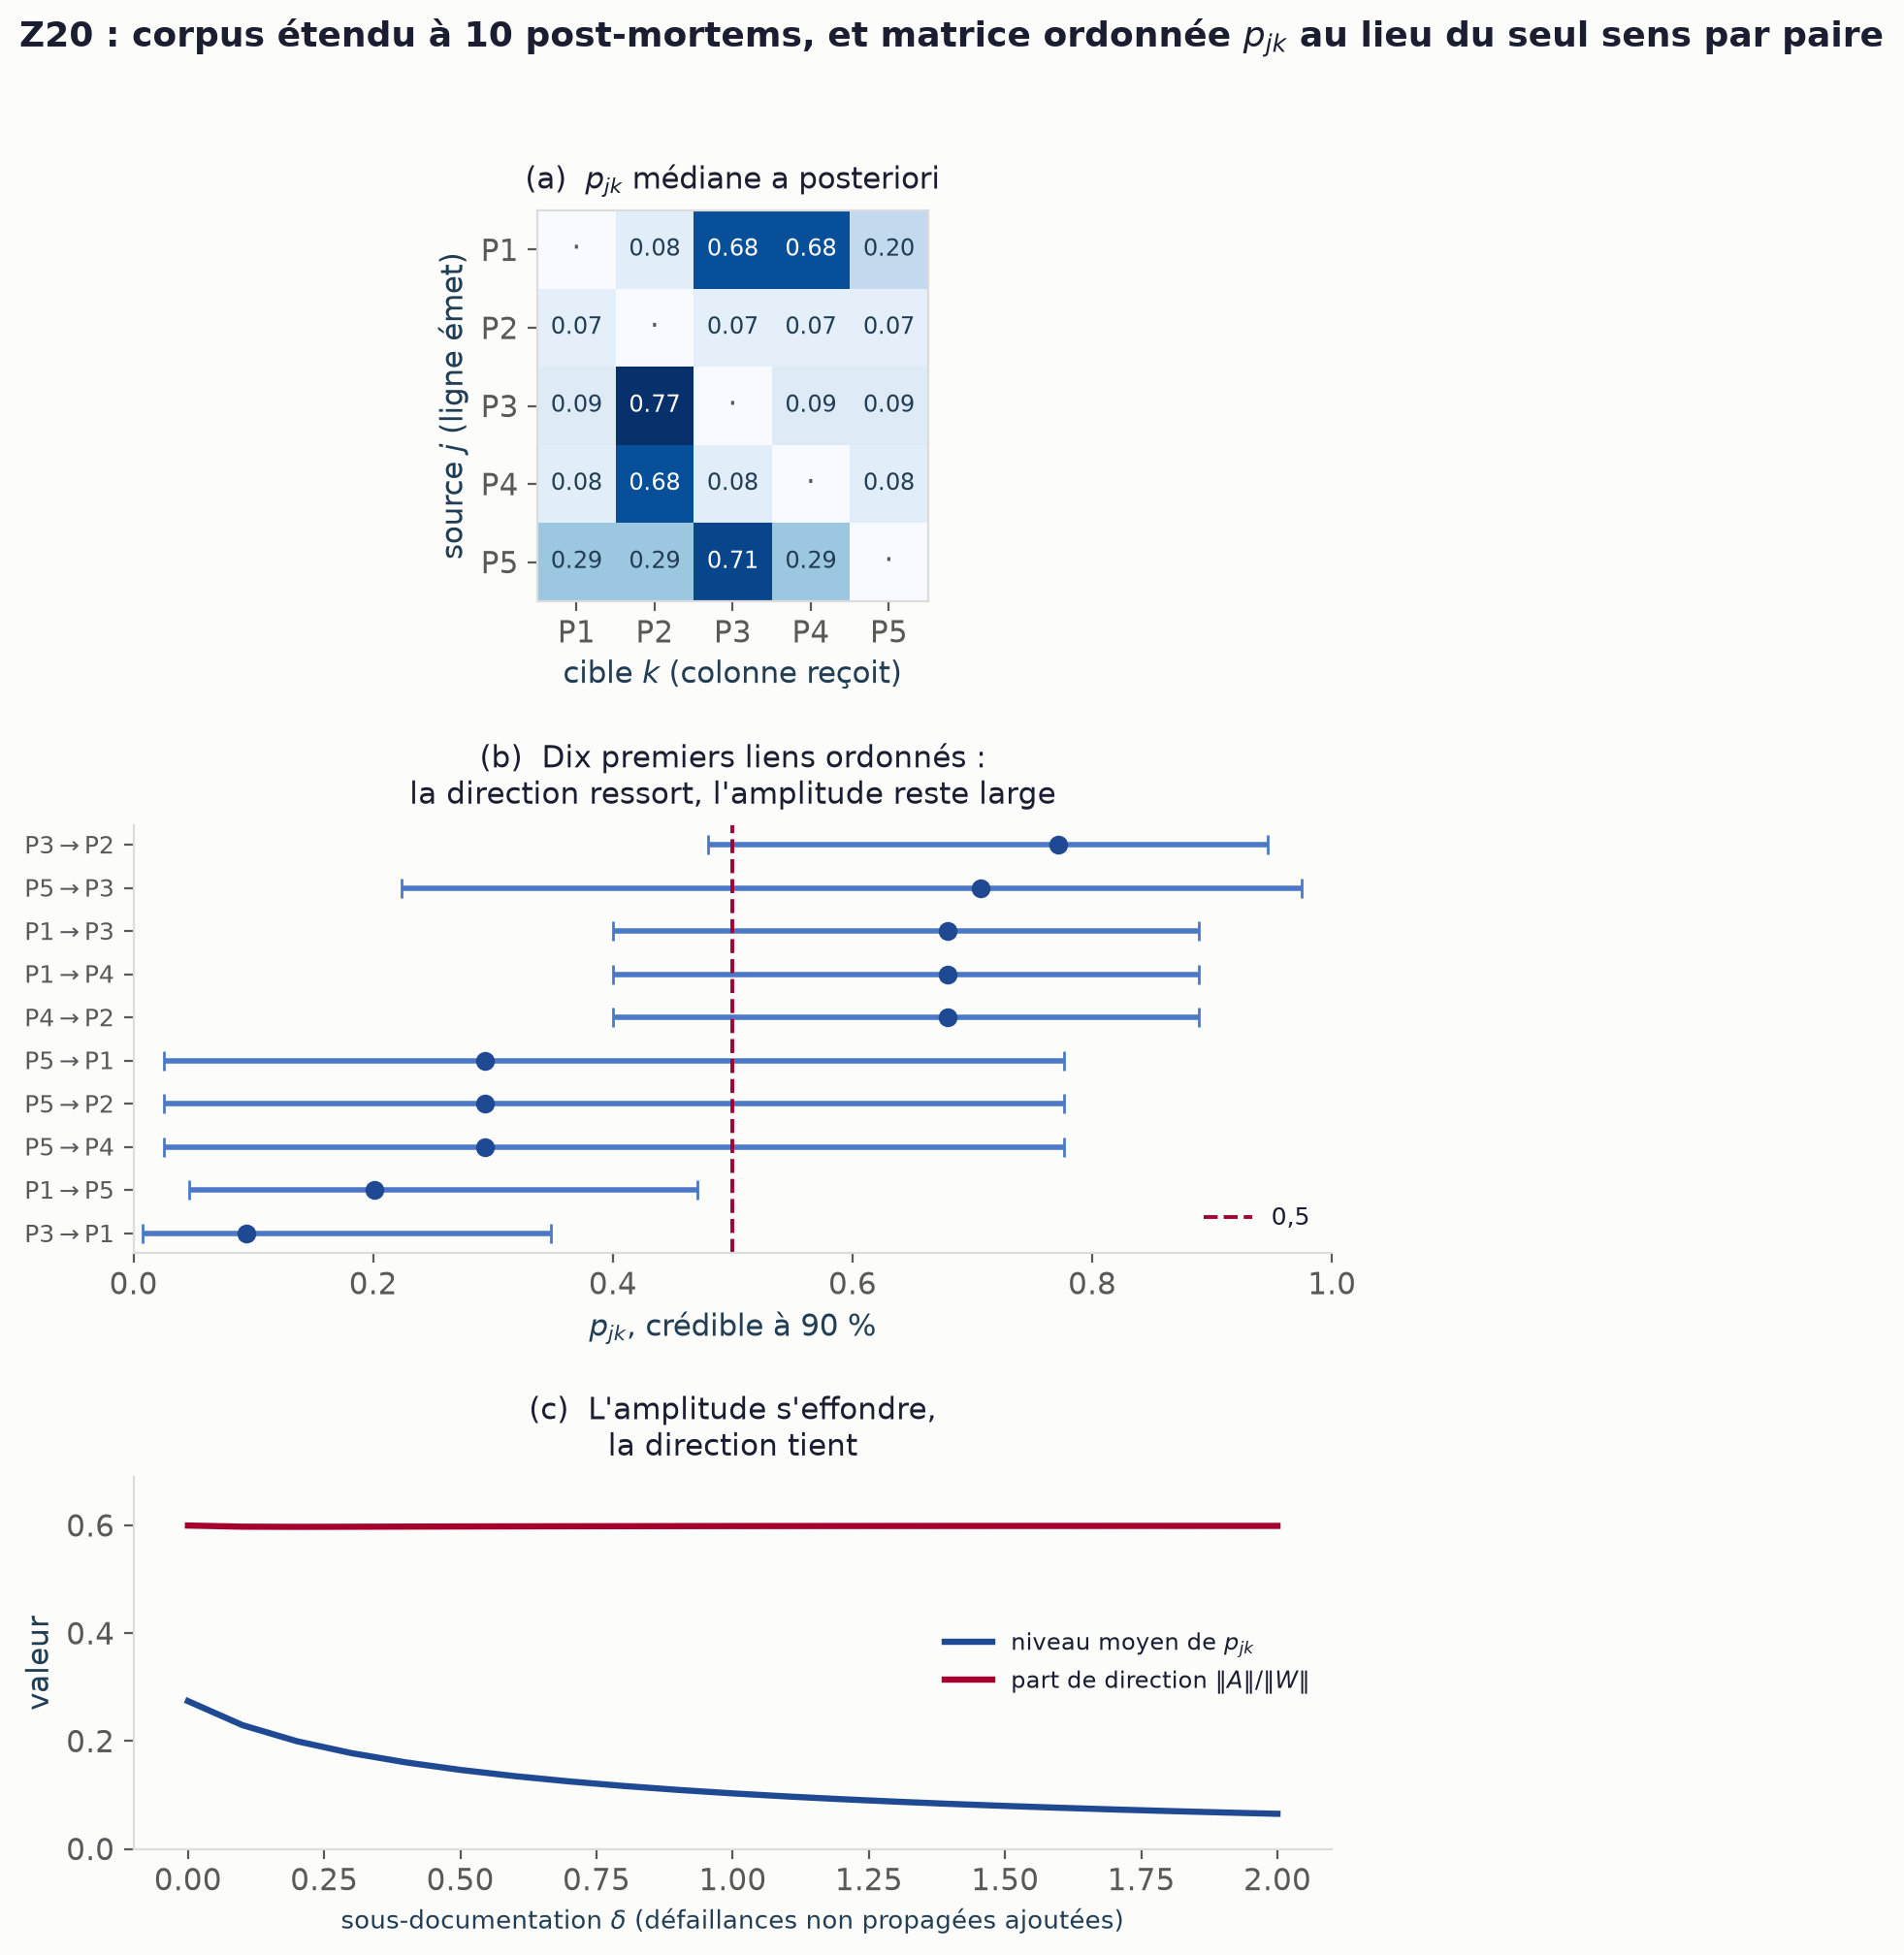
\includegraphics[height=0.80\textheight]{Z20_corpus_etendu_pij.png}
\end{center}
\end{frame}

% =====================================================================
\section*{G. La décision sur l'élicitation}

\begin{frame}{Je propose de renoncer à l'élicitation}
\scriptsize
\begin{block}{Pourquoi maintenant}
Le protocole exige $16$ questions par expert, dont $10$ graines à vérité connue, et écarte tout
expert incomplet. Avec le calendrier et le nombre de répondants réalistes, on obtiendrait une
à deux réponses exploitables. \textbf{Une agrégation de Cooke à deux experts n'a aucun pouvoir
de calibration}, et le chapitre~10 montre déjà qu'un panel biaisé déplace le SCR de
$777$~M\euro{} sans que rien ne le signale au lecteur. Une élicitation faible serait un
passif, pas un actif.
\end{block}
\vspace{-1mm}
\begin{columns}[t]
\begin{column}{0.48\linewidth}
\textbf{Ce que cela coûte, exactement}
\begin{itemize}\itemsep0pt
\item Le \textbf{départage P1 / P4}, donc l'ordre de remédiation entre les deux piliers de
      tête.
\item Le \textbf{resserrement} de la bande.
\end{itemize}
\emph{Et rien d'autre.}
\end{column}
\begin{column}{0.48\linewidth}
\textbf{Ce qui ne bouge pas}
\begin{itemize}\itemsep0pt
\item Le socle $5\,275$~M\euro, sans aucun paramètre non identifiable.
\item Les bornes $[6\,858;8\,697]$.
\item $\mathbf{79\,\%}$ du capital, déjà fixé.
\end{itemize}
\end{column}
\end{columns}
\vspace{1mm}
\begin{block}{Ce qui la remplace, et qui existe déjà}
Le \textbf{corpus documentaire} (slide précédente, $z=+5{,}12$), le \textbf{bayésien conjugué}
qui formalise la direction \emph{sans aucun prior d'expert}, l'\textbf{échelle de repli} sur
$u_{ij}$ dont le cran de rang~$1$ capte $74\,\%$ de la direction et resserre les bornes de
$25\,\%$, et les \textbf{ancrages réglementaires} (ESA, BCE) déjà utilisés.
\end{block}
\vspace{-1mm}
{\scriptsize Sources : scripts~\texttt{29}, \texttt{31}, \texttt{34}, \texttt{54}
et~\texttt{59}.}
\end{frame}

% =====================================================================
% CINQ NOMBRES DE CETTE SLIDE SONT HORS SCRIPT, ET CHACUN POUR UNE RAISON PROPRE. Le harnais
% les remonte comme non confirmes, ce qui est correct : ils ne viennent d'aucun calcul.
%   0,572 : la valeur FAUSSE du rayon spectral, citee ici justement parce qu'elle a ete
%           corrigee. Aucun script ne l'imprime, et c'est le resultat voulu.
%   30    : une CIBLE de corpus proposee, pas une mesure.
%   104, 126, 70 : comptes de pages et recommandation de l'Institut, metadonnees du document.
% A relire si ce compte de pages bouge : le corps a gagne deux pages le 10 aout avec la table
% des postures et les deux limites declarees au chapitre 13.
\begin{frame}{L'état du document, et les points bloquants}
\scriptsize
\begin{block}{La relecture complète est faite : dix-neuf chapitres, quinze défauts corrigés}
Les trois plus sérieux étaient invisibles à la lecture courante. Une \textbf{erreur numérique}
($\rho(W)$ valait $0{,}572$ au ch.~7 et $0{,}506$ au ch.~8 ; le calcul donne $0{,}506$). Une
\textbf{convention d'indices contradictoire} ($W_{jk}$ désignait la source dans la définition
de la cascade, la cible dans l'équation structurelle). Des \textbf{labels en double} faisant
pointer l'annexe de démonstrations vers le mauvais chapitre.
\end{block}
\begin{columns}[t]
\begin{column}{0.485\linewidth}
\textbf{Ce qui dépend d'autres que moi}
\begin{itemize}\itemsep0pt
\item Le \textbf{registre d'externalisation}, ingestion prête.
\item Le \textbf{choix de posture}, prédictif ou robuste, à trancher avec Caroline.
\item Un \textbf{second codeur en aveugle} : cela ne demande pas un expert, juste un lecteur
      attentif.
\end{itemize}
\end{column}
\begin{column}{0.485\linewidth}
\textbf{Ce que je propose ensuite}
\begin{itemize}\itemsep0pt
\item Porter le corpus de $10$ à $30$ rapports : le registre d'\emph{enforcement} de la FCA
      est public et dense en entités réglementées.
\item Vérifier le \textbf{format} : $104$ pages de corps et $126$ au total, contre les $\sim70$
      de corps recommandés par l'Institut.
\end{itemize}
\end{column}
\end{columns}
\vspace{1mm}
\begin{block}{Ce qu'il faut retenir de ce point}
\textbf{Le niveau bouge dans la bande, l'ordre des piliers ne bouge pas.} Trois choses de plus
sont passées du statut \emph{déclaré} au statut \emph{mesuré} cette semaine, le mémoire ne
dépend plus d'une élicitation qui n'aura pas lieu, et les trois échelles du capital ne peuvent
plus être confondues : \textbf{le pont entre elles est calculé, imprimé, et recalculé à chaque
exécution}.
\end{block}
\end{frame}

\end{document}
